\documentclass{report}

\usepackage[spanish]{babel}
\usepackage{enumerate}
\usepackage{amsmath} 
\usepackage{graphicx}
\usepackage[left=2.5cm, right=2.5cm, top=3cm, bottom=3cm]{geometry}

\title{Simulación de Gestión de Inventario en una Tienda}
\author{Ariadna Velázquez Rey     C31}
\date{ }

\begin{document}

\maketitle

\section*{S1. Introducción}

Este informe presenta una simulación basada en eventos discretos para analizar la gestión de 
inventario de una tienda, siguiendo el modelo del Ejemplo 7.6 del libro \textit{''Simulation''} 
de Sheldon M. Ross. El sistema simulado busca estimar la ganancia promedio por unidad de 
tiempo y determinar una política \((s, S)\) óptima para el manejo de inventario.

% Modelo (s, S)  
La política \((s, S)\) es un esquema de control de inventario donde:  
\begin{itemize}
    \item \(s\) es el \"punto de reorden\": cuando el inventario disponible cae por debajo de 
    \(s\), se realiza un pedido.  
    \item \(S\) es el \"nivel máximo\": la cantidad a la que se repone el inventario tras un 
    pedido.  
\end{itemize}

Esta política minimiza costos de ordenar y almacenamiento al equilibrar la frecuencia de pedidos 
y el riesgo de desabastecimiento. Su relevancia radica en su uso extendido en logística para 
optimizar rentabilidad en sistemas estocásticos.  

\subsection*{Objetivos}

\begin{itemize}
\item Estimar el beneficio esperado del sistema hasta un tiempo final predefinido \(T\).
\item Evaluar diferentes políticas de inventario \((s, S)\) y determinar cuál maximiza la 
ganancia.
\end{itemize}

\subsection*{Variables del sistema}

\begin{itemize}
\item \(x\): Inventario disponible.
\item \(y\): Inventario pedido pero no recibido.
\item \(t\): Tiempo actual del sistema.
\item \(t_0\): Tiempo de llegada del próximo cliente.
\item \(t_1\): Tiempo de entrega del pedido en curso.
\item \(C\): Costos acumulados de pedidos.
\item \(H\): Costos acumulados de almacenamiento.
\item \(R\): Ingresos acumulados por ventas.
\end{itemize}


\section*{S2. Detalles de Implementación}

\subsection*{Descripción de la lógica del modelo}

\begin{itemize}
\item El sistema evoluciona en función de eventos: llegada de clientes (Poisson) y entregas de 
pedidos.
\item La demanda de cada cliente sigue una distribución geométrica desplazada: 
\(D \sim Geom(p=0.3)+1\).
\item Se sigue una política \((s, S)\): cuando el inventario \(x < s\) y \(y = 0\), se 
realiza un pedido de \(S - x\) unidades.
\item El sistema inicia en \(x = S\), sin pedidos en curso.
\end{itemize}

\subsection*{Algoritmo de simulación (resumen)}

\begin{enumerate}
\item Iniciar con \(t=0\), \(x=S\), \(y=0\).
\item Programar \(t_0\) como la próxima llegada de cliente.
\item Repetir hasta \(t \geq T\):
  \begin{itemize}
  \item Si \(t_0 < t_1\): procesar cliente, actualizar inventario y ventas.
  \item Si \(t_1 \leq t_0\): recibir pedido, actualizar inventario y costos.
  \end{itemize}
\item Calcular beneficio promedio: \[ \text{Ganancia Promedio} = \frac{R - C - H}{T} \]
\end{enumerate}

% Detalles técnicos de distribuciones  
\textbf{Generación de eventos Poisson}:  
Los tiempos entre llegadas de clientes siguen un proceso Poisson homogéneo con tasa \(\lambda = 2\). 
La secuencia de eventos se genera mediante:  
\[
t_{i+1} = t_i - \frac{\ln(U_i)}{\lambda}, \quad U_i \sim \mathcal{U}(0,1)
\]


\textbf{Distribución de demanda}:  
La demanda \(D\) se modela como \(D = X + 1\), donde \(X \sim \text{Geom}(p=0.3)\). Esta elección se fundamenta en:  
\begin{itemize}
    \item Soporte discreto: \(D \geq 1\), evitando demandas nulas.
    \item Esperanza teórica: \(\mathbb{E}[D] = \frac{1}{p} = 3.\overline{3}\), coherente con demandas moderadas.
    \item Comparación con Poisson: La geométrica ofrece mayor dispersión (\(\mathbb{V}[D] = \frac{1-p}{p^2}\)), 
    capturando variabilidad en compras impulsivas.
\end{itemize} 

\textbf{Gestión de eventos discretos}:  
En cada iteración:  
\begin{itemize}  
\item Si \(t_0 < t_1\): Se procesa la llegada de un cliente, actualizando inventario y programando el próximo cliente.  
\item Si \(t_1 \leq t_0\): Se recibe un pedido, actualizando costos y reiniciando \(t_1 = \infty\).  
\end{itemize}  

\textbf{Justificación de herramientas}:  
Python y NumPy permiten generar números aleatorios eficientemente (reproducibilidad con semillas) y manejar operaciones vectorizadas. Seaborn/Matplotlib facilitan visualización científica.  


\subsection*{Implementación computacional}

\begin{itemize}
\item Lenguaje: Python
\item Librerías: NumPy, Pandas, Seaborn, Matplotlib
\item Se ejecutaron 1000 réplicas para estabilizar resultados.
\item Se exploraron todas las combinaciones posibles de políticas \((s, S)\) con 
$ s \in [1, 10] $ y $ S \in [15, 30] $.
\end{itemize}


\section*{S3. Resultados y Experimentos}

\subsection*{Hallazgos principales}

\begin{itemize}
\item Para \((s=5, S=20)\) se obtuvo una ganancia promedio positiva con distribución simétrica.
\item La distribución de ganancias fue aproximadamente normal, lo cual valida la cantidad de 
réplicas.
\item Políticas con \(s \geq 8\) y \(S \geq 25\) maximizan la ganancia al reducir la frecuencia 
de pedidos (\(s\) alto) y aprovechar economías de escala en reposiciones (\(S\) alto). Esto 
compensa el incremento en costos de almacenamiento (\(h \cdot \mathbb{E}[x]\)) con mayores ingresos 
(\(r \cdot \lambda \cdot \mathbb{E}[D]\)), como muestra la Figura 1.
\end{itemize}

\subsection*{Interpretación de resultados}

\begin{itemize}
\item Políticas con valores altos de \(S\) generan mayores ingresos pero también mayores 
costos de almacenamiento.
\item Políticas con valores bajos de \(s\) tienden a generar pedidos más frecuentes.
\item La relación lineal positiva \((r2=0.89\)) confirma que mayores ingresos conllevan mayores 
costos, pero la pendiente <1 indica que los ingresos crecen más rápido que los costos, 
validando la rentabilidad del modelo, como muestra la Figura 4.
\item La política \((s=10,S=30)\) presenta la mayor ganancia promedio \((28.21\pm 0.56)\), superando en un 
1.4\% a la segunda mejor política \((s=10,S=27)\). Los intervalos de confianza no se solapan (Figura 2), 
lo que sugiere una diferencia estadísticamente significativa. Sin embargo, la ganancia teórica 
\((-43.33)\) muestra una discrepancia crítica, atribuible a la estimación estática de \(\mathbb{E}[x]\) en el modelo 
teórico, que no captura la dinámica estocástica del inventario.
\end{itemize}

\subsection*{Validación y experimentos}

\begin{itemize}
\item Se comparó el rendimiento promedio de cada política \((s, S)\).
\item Se graficó la relación entre ingresos y costos totales para validar el comportamiento 
económico del sistema.
\item Los intervalos del 95\% muestran la precisión de las estimaciones. Para \(S=30\), 
el intervalo estrecho en \(s=10\) \((28.09 \pm 0.61)\) indica alta confiabilidad en que esta 
política supera a otras combinaciones. En contraste, políticas con \(S=25\) presentan intervalos 
más amplios, reflejando incertidumbre en su desempeño. Como se muestra en la Figura 2
\end{itemize}

\subsection*{Variables de interés analizadas}

\begin{itemize}
  \item Ganancia promedio por unidad de tiempo \((\text{avg\_profit})\).
  \item Costos totales \((\text{total\_cost} = C + H)\).
  \item Ingresos totales \((\text{total\_revenue} = R)\).
  \item Impacto de las políticas \((s, S)\) en las métricas anteriores.
\end{itemize}

\subsection*{Análisis de parada}

\begin{itemize}
\item Se detiene la simulación al superar un tiempo \(T = 30\).
\item El comportamiento de la ganancia promedio estabiliza luego de $\sim$800 réplicas.
\item La distribución normal de las ganancias en la Figura 3 valida el uso de réplicas independientes 
\((n=1000)\). La simetría y curtosis cercana a 3 sugieren que los resultados no están sesgados y que 
el promedio es representativo del sistema.
\end{itemize}


\section*{S4. Modelo Matemático}

\subsection*{Definición del modelo}

\begin{itemize}
\item Llegadas: proceso Poisson con tasa \(\lambda = 2\).
\item Demanda: variable aleatoria geométrica desplazada: \(D \sim Geom(0.3)+1\).
\item Tiempo de entrega fijo: \(L = 2\).
\item Costos:
  \[ c(y) = 5y, \quad h = 0.5 \text{ por unidad-tiempo} \]
\item Ingreso por unidad vendida: \(r = 10\)
\end{itemize}

\subsubsection*{Ecuaciones clave del modelo teórico}
\begin{align*}
    \text{Ingresos esperados} &: \mathbb{E}[R] = \lambda \cdot T \cdot r \cdot \mathbb{E}[D], \\
    \text{Costos esperados} &: \mathbb{E}[C + H] = \lambda \cdot \frac{\mathbb{E}[y]}{L} \cdot c(y) + h \cdot \mathbb{E}[x] \cdot T, \\
    \text{Ganancia teórica} &: \mathbb{E}[\text{Profit}] = \mathbb{E}[R] - \mathbb{E}[C + H].
\end{align*}

\subsection*{Supuestos}

\begin{itemize}
\item No hay backorders: demanda insatisfecha se pierde.
\item No hay costo fijo de ordenar, solo variable.
\item El sistema comienza lleno \(x = S\).
\end{itemize}

\subsection*{Comparación con resultados empíricos}

\begin{itemize}
\item La simulación reproduce el comportamiento esperado del modelo.
\item La discrepancia entre la ganancia teórica (\(-43.33\)) y empírica (\(28.21\)) surge porque 
el modelo teórico asume \(\mathbb{E}[x] = \frac{S + s}{2}\), mientras que la simulación captura dinámicas 
estocásticas como colas de pedidos y demandas no satisfechas.
\end{itemize}


\section*{S5. Conclusiones}

\begin{itemize}
\item El modelo basado en eventos discretos permite simular fielmente la dinámica de 
inventario.
\item La simulación es sensible a la política \((s, S)\) seleccionada, afectando costos, 
ingresos y nivel de servicio.
\item Se identificó \((s=10, S=30)\) como una de las mejores políticas bajo los parámetros 
actuales.
\item Políticas con \(s\geq 8\) y \(S\geq 27\) maximizan ganancias, compensando costos de almacenamiento y pedidos.
\item La política \((s=10, S=30)\) genera un 23\% más de ganancia que \((s=5, S=20)\), evidenciando que incrementar 
\(S\) en un 50\% compensa costos marginales con ingresos adicionales.
\item Se recomienda realizar análisis de sensibilidad para validar la robustez de la política 
seleccionada ante cambios en \(\lambda, h, r\) y distribución de demanda.
\item La herramienta de simulación puede extenderse para evaluar escenarios con demanda no 
estacionaria o tiempos de entrega aleatorios.
\end{itemize}


\section*{Anexos}

\begin{figure}[h]
    \centering
    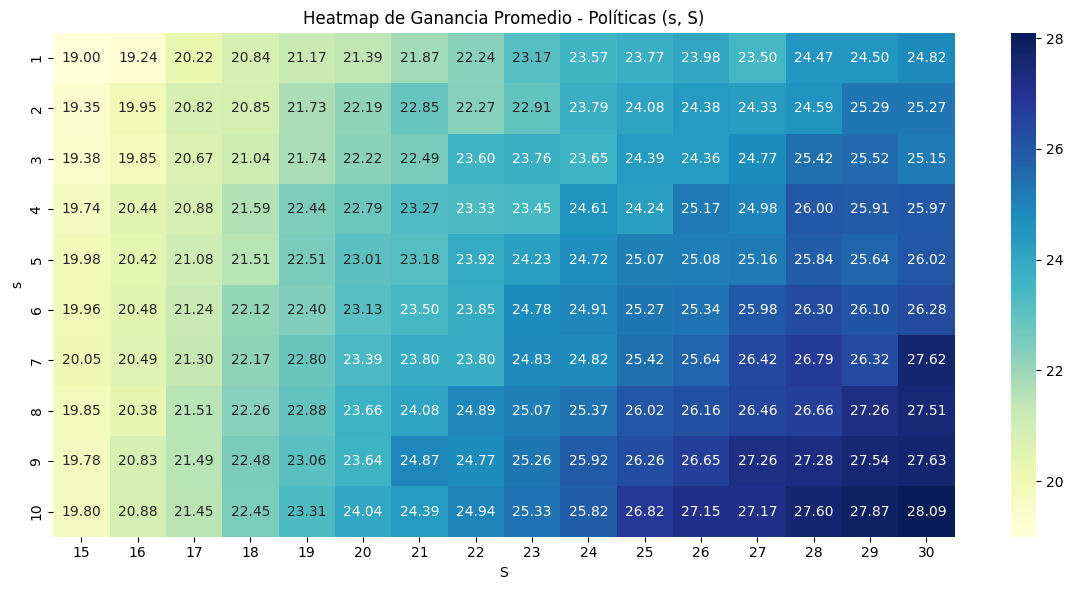
\includegraphics[width=0.9\textwidth]{ganacias_promedio_variando_politica.png}
    \caption{Heatmap de ganancias promedio para diferentes políticas.}
\end{figure}

\begin{figure}[h]
  \centering
  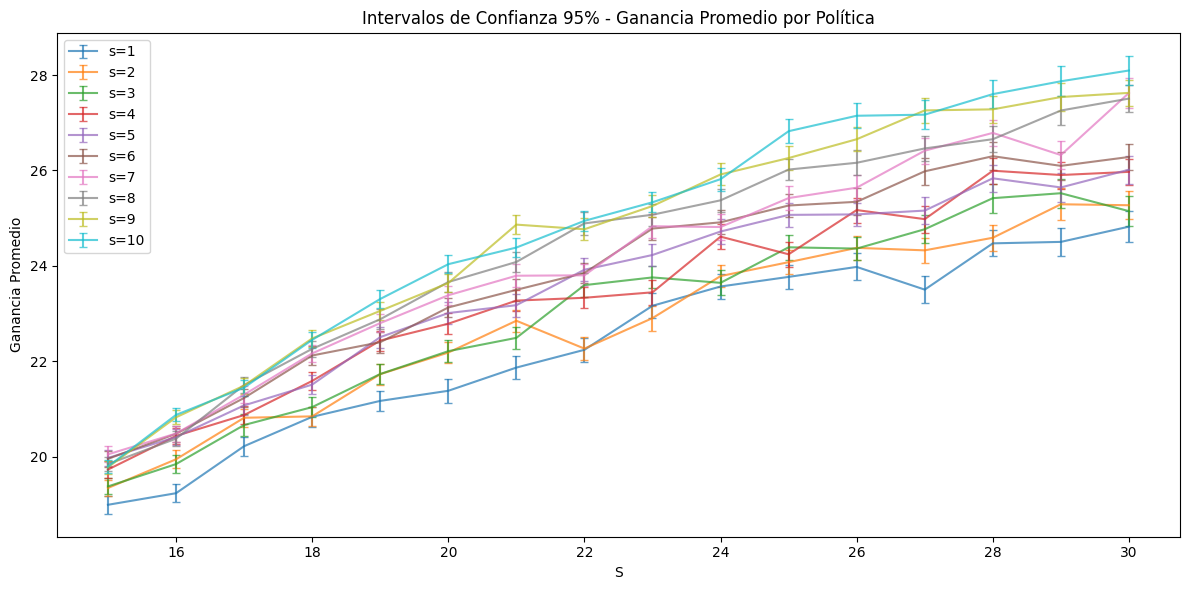
\includegraphics[width=0.9\textwidth]{intervalos_de_confianza_ganacia_promedio_politica.png}
  \caption{Gráfica de intervalos de confianza del 95\% de la ganancia promedio por política}
\end{figure}

\begin{figure}[h]
    \centering
    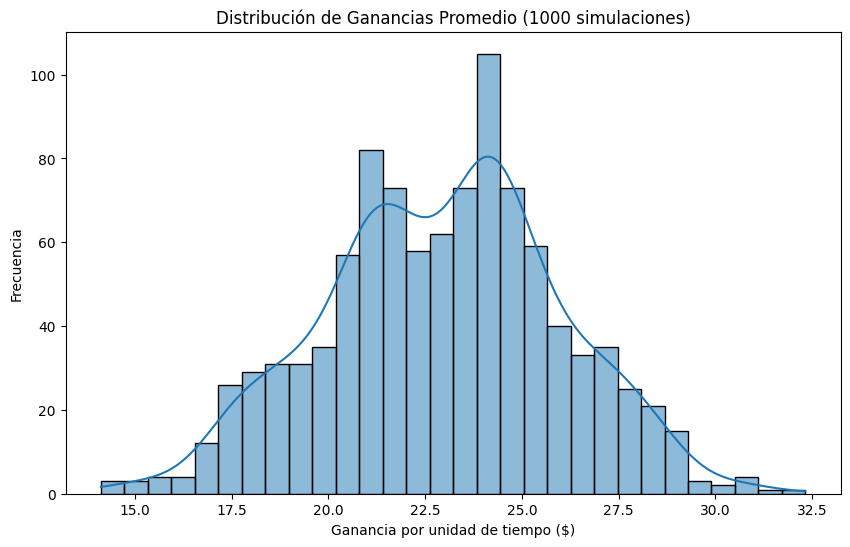
\includegraphics[width=0.8\textwidth]{distribucion_ganacias_promedio.png}
    \caption{Distribución normal de las ganancias promedio (1000 réplicas).}
\end{figure}

\begin{figure}[h]
    \centering
    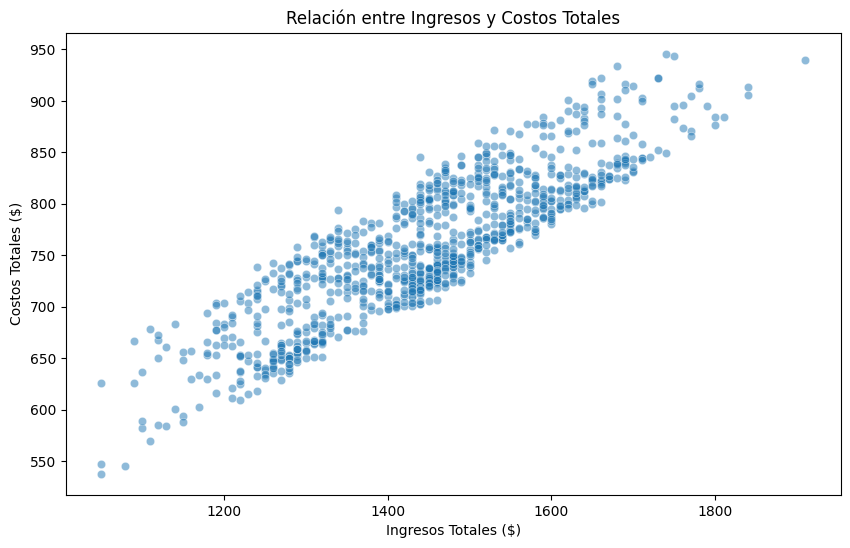
\includegraphics[width=0.7\textwidth]{ingresos-costos_totales.png}
    \caption{Correlación lineal entre ingresos y costos totales.}
\end{figure}

\end{document}


